\documentclass{article}
\usepackage{cite}
\usepackage[utf8]{inputenc}
\newcommand\independent{\protect\mathpalette{\protect\independenT}{\perp}}
\def\independenT#1#2{\mathrel{\rlap{$#1#2$}\mkern2mu{#1#2}}}
\title{Report for Comp Exam}
\author{Siyuan Zhao}
\date{March 2017}

\usepackage[linesnumbered,ruled]{algorithm2e}
\usepackage{amsmath, mathtools}
\usepackage{amsfonts}
\begin{document}

\maketitle

\section{Problem Setup}
Let $\mathcal{T}$ be the set of proposed interventions we wish to
consider, $X$ the set of participants, and $Y$ the set of possible
outcomes. For each proposed intervention $t \in \mathcal{T}$, let
$Y(t) \in Y$ be the potential outcome for $x$ when x is assigned to
the intervention $t$. In randomized control trial (RCT) and observed
study, only one outcome is observed for a given participant $x$; even
if the participant is given an intervention and later the other, the
participant is not in the same state.

In the binary intervention set, there are two possible interventions
$\mathcal{T} = \left \{  0, 1 \right \}$, where intervention 1 is
often referred as the "treated" and intervention 0 is the "control."
Given a sample of subjects and a treatment, each subject has a pair of
potential outcomes: $Y_i(0)$ and $Y_i(1)$, the outcomes under the
control and the treatment, respectively. Let $t$ be an indicator
variable denoting the treatment received ($t = 0$ for the control and
$t=1$ for the treatment). Only one outcome, $Y_i (Y_i=t\cdot Y_i(1) +
(1-t) \cdot Y_i(0))$, is observed for the
subject $i$.

The individual treatment effect (ITE) can be defined to
be $Y_i(1) - Y_i(0)$. The average treatment effect (ATE) is defined to
be $E[Y_i(1) - Y_i(0)]$. The ATE is the average treatment effect, at
the population level, of moving an entire population from the control
to the treatment. A related measure of treatment effect is the average
treatment effect for the treated (ATT) \cite{imbens2004}. The ATT is
defined as $E[Y(1)-Y(0) \mid t=1]$. The ATT is the average effect of
treatment on those subjects who ultimately received the treatment. In
an RCT these tow measures of treatment effects coincide because, due
to randomization, the treated population will not, on average, differ
systematically from overall population.

\subsection{Randomized Controlled Trials}
In RCTs, treatment is assigned by randomization. As a consequence of
randomization, an unbiased estimate of the ATE can be directly
computed from the data. An unbiased estimate of the ATE is
$E[Y_i(1)-Y_i(0)]=E[Y(1)] - E[Y(0)]$. This definition allows one to
define the ATE in terms of a difference in means (continuous outcomes)
or a difference in proportions (binary outcomes).

\subsection{Observational Studies}
An observational study has the same intent as a randomized experiment:
to estimate a causal effect. However, an observational study differs
from a RCT in one design issue: the use of randomization to allocate
units to treatment and control groups.

In observational studies, the treated subjects often differ
systematically from untreated subjects. In general, $E[Y(1)\mid t=1]
\neq E[Y(1)]$ holds. Thus, an unbiased estimate of the average
treatment effect cannot be obtained by directly comparing outcomes
between the two treatment groups.

\subsection{Strong Ignorability}
The treatment assignment is defined to be strongly ignorable
\cite{rosenbaum1983central} if the following two conditions hold: 1).
$(Y(1), Y(0)) \independent t\mid X$ and 2). $0 < \Pr (t=1 \mid X) <
1$. The first condition says that treatment assignment is independent
of the potential outcomes conditional on the observed baseline
covariates. The second condition says that every subject has a nonzero
probability to receive either treatment. The aforementioned first
condition is also referred to as the "no unmeasured confounders"
assumption that all variables that affect treatment assignment and
outcome have been measured.
\section{Random Causal Forest}
\cite{wager2015estimation} proposed random causal forest (RCF) to
infer treatment effect. From the conceptual point of view, trees and forests can be viewed as
nearest neighbor methods with an adaptive neighborhood metric. Given
observed independent samples $(X_i, Y_i, W_i)$, a causal tree is first
built by recursively splitting the feature space until all samples are
partitioned into a set of leaves $L$, each of which contains a few
training samples. Then, for a data point $x$, the predicted outcome $\hat{\mu}(x)$
is evaluated by identifying the leaf $L(x)$ containing $x$ and
calculating

$$\hat{\mu} = \frac{1}{\left | \left \{ i: X_i \in L(x) \right \}
  \right |} \sum_{\left \{ i: X_i \in L(x) \right \}} Y_i$$

Given a test point $x$, the closest points to $x$ are those fall in the same
leaf as it. The authors believe that the leaf is small enough that the
responses $Y_i$ are roughly identically distributed. Then the
treatment effect $\hat{\tau}$ for any $x \in L(x)$ is estimated as
following:

\begin{align*}
\hat{\tau}(x) & = \frac{1}{\left | \left \{ i: W_i=1, X_i \in L(x) \right \}
  \right |} \sum_{\left \{ i: W_i = 1, X_i \in L(x) \right \}} Y_i \\ & - \frac{1}{\left | \left \{ i: W_i=0, X_i \in L(x) \right \}
  \right |} \sum_{\left \{ i: W_i = 0, X_i \in L(x) \right \}} Y_i
\end{align*}
RCF assumes that
there is overlapping in the data, i.e., for some $\epsilon > 0$ and
all $x \in \left [ 0, 1\right ]^d$,

$$\epsilon < \mathbb{P}\left [ W=1 \mid X=x \right ] < 1-\epsilon$$

This condition effectively guarantees that, for large enough $n$,
there will be enough treatment and control units near any test point
$x$ for local methods to work.

\section{Individualized Treatment Rules}
In experiments, we observe a triplet $(\mathbf{x}, t, y)$ from each
participant, where $\mathbf{x}=(x_1, x_2, \ldots, x_n)^T \in
\mathcal{X}$ denotes the participant's covariates, $t \in \mathcal{T}
= {-1,1}$ denotes the treatment assignment, and $y \in Y$ is the
observed outcome, also called the "reward" in the literature on
reinforcement learning. Note that $t=-1$ means the control in the
context of ITR. Let $p(t|x)$ be the probability of assigning the participant
with covariates $\mathbf{x}$ to the intervention $t$.

An individual treatment rule (ITR) $d: X \rightarrow \mathcal{T}$ is a deterministic decision
rule from subject $x$ into the intervention space $\mathcal{T}$. The
value of $d$ satisfies
$$V(d) = E \left [ \frac{y}{p(t|x)}\mathbb{I}_{t=d(\mathbf{x})}\right
],$$
where $\mathbb{I}(\cdot)$ is an indicator function. An optimal ITR, $d^{*}$, is a rule that has the maximal value such
that,

$$d^{*} \in \operatorname*{arg\,max}_d V(d).$$
Finding $d^{*}$ is equivalent to minimizing the following equation:
\begin{equation} \label{eq:d_min}
d^{*} \in \operatorname*{arg\,min}_d E \left [
  \frac{y}{p(t|x)}\mathbb{I}_{t \neq d(\mathbf{x})}\right
]
\end{equation}

Assume that the observed data $\left \{
  (\mathbf{x}_i,t_i,y_i),~i=1,\ldots , n \right \}$ are collected
independently. For any decision function $f(\mathbf{x})$, let
$d_f(\mathbf{x}) = sign(f(\mathbf{x}))$ be the associated rule, where
$sign(u) = 1$ for $u > 0$ and $-1$ otherwise. The particular choice of
the value of $sign(0)$ is not important. With the observed data, the
weighted classification error in Equation \ref{eq:d_min} can be approximated by
the empirical risk

\begin{equation} \label{eq:d_empirical_min}
  \frac{1}{n}\sum_{i=1}^{n}\frac{y_i}{p(t_i|x_i)}\mathbb{I}_{t_i \neq
    d_f(\mathbf{x_i})} .
\end{equation}

It is well known that empirical risk minimization for a classification
problem with the $0-1$ loss function is an NP-hard problem. To solve
this difficulty, outcome weighted learning (OWL) is proposed by
\cite{zhao2012estimating} using the hinge loss function and the
regularization technique. In other words, instead of minimizing
Equation~\ref{eq:d_empirical_min}, OWL aims to minimize

\begin{equation} \label{eq:d_owl_empirical_min}
  \frac{1}{n}\sum_{i=1}^{n}\frac{y_i}{p(t_i|x_i)}(1-t_if(\mathbf{x}_i))_{+}+\lambda\left
    \| f \right \|^2 ,
\end{equation}
where $(u)_+=\max(u,0)$ is the positive part of $u$, $\left \| f
\right \|$ is some norm for $f$, and $\lambda$ is a tuning parameter
controlling the trade-off between empirical risk and complexity of the
decision function $f$.
\section{Bayesian Optimization}
Bayesian optimization is a sequential design strategy for global optimization of black-box functions that does not require derivatives. Since the objective function is unknown, the Bayesian
strategy is to treat it as a random function and place a prior over it. The prior captures our beliefs about the behaviour of the
function. After gathering the function evaluations, which are treated
as data, the prior is updated to form the posterior distribution
over the objective function. The posterior distribution, in turn, is
used to construct an acquisition function that determines what the
next query point should be. Examples of acquisition functions includes
probability of improvement, expected improvement, Bayesian expected
losses, upper confidence bounds (UCB), Thompson sampling and mixtures
of these. They all trade-off exploration and exploitation so as to
minimize the number of function queries. As such, Bayesian
optimization is well suited for functions that are very expensive to evaluate.

In summary, Bayesian optimization is the combination of two main components: a surrogate model which captures all prior and observed information and a decision process which performs the optimal action, i.e.: where to sample next, based on the previous model.

However, the Gaussian process (GP) is the most popular model due to
its accuracy, robustness and flexibility, because Bayesian
optimization is mainly usesd in blck-box scenarios. The range of
applicaility of a Gaussian process is defined by its kernel function,
which sets the family of functions that is able to represent through
the reproducing kernel Hilbert space (RKHS). In BO, attributes of the
GP such as mean and variance are used to sample successive points. It
is suitable for situations where cost function is costly to evaluate
and MCMC techniques would not work.

\subsection{Sequential method}
The sequential approach is independent of the choice of prior and of
the likelihood function and depends only on the assumption of i.i.d
data. Sequential methods make use of observations one at a time, or in
small batches, and then discard them before the next observations are
used. They can be used, for example, in real-time learning scenarios
where a steady stream of data is arriving, and predictions must be
made before all of the data is seen. Because they do not require the
whole data set to be stored or loaded into memory, sequential methods
are also useful for large data sets.

\section{Propensity Score Matching}
A propensity score is the probability of a unit (e.g., student,
classroom, school) being assigned to a particular treatment given a
set of observed covariates. Propensity scores are used to reduce
selection bias by equating groups based on these covariates.

Propensity score matching (PSM) entails forming matched sets of treated and
untreated subjects who share a similar value of the propensity
score. PSM allows one to estimate the average treatment effect for the
treated (ATT). The ATT is the average effect of treatment on those
subjects who ultimately receive the treatment. The most common
implementation of PSM is one-to-one or pair matching, in which pairs
of treated and untreated subjects are formed, such that matched
subjects have similar values of the propensity score. Once a matched
sample has been formed, the treatment effect can be estimated by
directly comparing outcomes between treated and untreated subjects in
the matched sample. If the outcome is continuous, the effect of
treatment can be estimated as the difference between the mean outcome
for treated subjects and the mean outcome for untreated subjects in
the matched sample. If the outcome is binary, the effect of treatment
can be estimated as the difference between the proportion of subjects
experiencing the event in each of the two groups (treated
vs. untreated) in the matched sample.

Suppose that we have a binary treatment $T={0,1}$, an outcome $Y$, and
background variables $X$. The propensity score is defined as the
conditional probability of treatment given background variables:

$$p(x):= \Pr(T=1 \mid X=x)$$

Let $Y(0)$ and $Y(1)$ denote the potential outcomes under the control
and the treatment, respectively.

The possibility of bias arises because the apparent difference in outcome between these two groups of units may depend on characteristics that affected whether or not a unit received a given treatment instead of due to the effect of the treatment per se. In randomized experiments, the randomization enables unbiased estimation of treatment effects; for each covariate, randomization implies that treatment-groups will be balanced on average, by the law of large numbers. Unfortunately, for observational studies, the assignment of treatments to research subjects is typically not random. Matching attempts to mimic randomization by creating a sample of units that received the treatment that is comparable on all observed covariates to a sample of units that did not receive the treatment.

The analysis of a propensity score matched sample can mimic that of an
RCT: one can directly compare outcomes between the treated and control
subjects within the propensity score matched sample. 
\section{Gaussian Processes}
Bayesian algorithms do not attempt to identify ‘best-fit’ models of the data (or similarly, make 'best guess' predictions for new test inputs). Instead, they compute a posterior distribution over models (or similarly, compute posterior predictive distributions for new test input). These distributions provide a useful way to quantify our uncertainty in model estimates, and to exploit our knowledge of this uncertainty in order to make more robust predictions on new test points.

Gaussian processes is the extension of multivariate Gaussian to infinite-sized collections of real-valued variables. In particular, this extension will allow us to think of Gaussian processes as distributions not just over random vectors but in fact distributions over random functions.

\subsection{Probability distributions over functions with finite domains}
Let $\mathcal{X} = \left \{ x_1, x_2, …, x_m \right \}$ be any finite set of elements. Consider the set $\mathcal{H}$ of all possible functions mapping from $\mathcal{X}$ to $\mathbf{R}$. For instance, one example of a function $f_0(\cdot) \in \mathcal{H}$ is given by

$$f_0(x_1)=5,~f_0(x_2)=2.3, \dotsb ,~f_0(x_{m-1})=-\pi,~f_0(x_m)=8.$$

Since the domain of any $f(\cdot) \in \mathcal{H}$ has only $m$ elements, we can always represent $f(\cdot)$ compactly as an $m$-dimensional vector, $\vec{f}=[f(x_1)~~f(x_2)~~...~~f(x_m) ]^T$. In order to specify a probability distribution over functions $f(\cdot) \in \mathcal{H}$, we must associate some "probability density" with each function in $\mathcal{H}$. One natural way to do this is to exploit the one-to-one correspondence between $f(\cdot) \in \mathcal{H}$ and their vector representation, $\vec{f}$. In particular, if we specify that $\vec{f}\sim \mathcal{N}(\vec{\mu},\sigma ^2I)$, then this in turn implies a probability distribution over functions $f(\cdot)$, whose probability density function is given by
$$p(h) = \prod_{i=1}^{m} \frac{1}{\sqrt{2\pi}\sigma}\mathrm{exp}(-\frac{1}{2\sigma ^2} (f(x_i)-\mu _i)^2)
$$

In the example above, we show that probability distributions over functions with finite domains can be represented using a finite-dimensional multivariate Gaussian distribution over function outputs $f(x_1),...,f(x_m)$ at a finite number of input points $x1, ..., x_m$

\subsection{Probability distributions over functions with infinite domains}
A stochastic process is a collection of random variables, $\left \{ f(x): x \in \mathcal{X} \right \}$, indexed by elements from some set $\mathcal{X}$, known as the index set. A Gaussian process is a stochastic process such that any finite sub-collection of random variables has a multivariate Gaussian distribution.

In particular, a collection of random variables $\left \{ f(x): x \in \mathcal{X} \right \}$ is said to be drawn from a Gaussian process with mean function $m(\cdot)$ and covariance function $k(\cdot , \cdot)$ if for any finite set of elements $x_1,...,x_m \in \mathcal{X}$, the associated finite set of random variables $f(x_1),...,f(x_m)$ have distribution,
$$\begin{bmatrix}
f(x_1)\\
\vdots \\
f(x_m) 
\end{bmatrix} \sim \mathcal{N} \left( 
\begin{bmatrix}
m(x_1)\\
\vdots \\
m(x_m) 
\end{bmatrix}, \begin{bmatrix}
k(x_1, x_1) & \cdots & k(x_1, x_m) \\
\vdots & \ddots & \vdots\\
k(x_m, x_1) & \cdots & k(x_m, x_m) \\
\end{bmatrix} 
\right).$$

We denote this using the notation,

$$f(\cdot) \sim \mathcal{GP}(m(\cdot), k(\cdot, \cdot)).$$

In general, any real-valued function $m(\cdot)$ is acceptable, but for $k(\cdot, \cdot)$, it must be the case that for any set of elements $x_1, \dotsc, x_m \in \mathcal{X}$, the resulting matrix
$$K = \begin{bmatrix}
k(x_1, x_1) & \cdots & k(x_1, x_m) \\
\vdots & \ddots & \vdots\\
k(x_m, x_1) & \cdots & k(x_m, x_m) \\
\end{bmatrix} $$
is a valid covariance matrix corresponding to some multivariate
Gaussian distribution. A standard result in probability theory states
that this is true provided that $K$ is positive semi-definite.

\section{Reproducing kernel Hilbert space}
In functional analysis, a reproducing kernel Hilbert space (RKHS) is a
Hilbert space of functions in which point evaluation is a continuous
linear functional. The representer theorem states that every function
in an RKHS that minimizes an empirical risk function can be written as
a linear combination of the kernel function evaluated at the training
points.

\section{Information Theory}
The entropy of the random variable $X$, where $p(X = x_i) = p_i$, is
defined as:
\begin{equation} \label{eq:entropy}
  \mathrm{H}[p] = -\sum_{i}p(x_i)\log p(x_i)
\end{equation}

Distributions $p(x_i)$ that are sharply peaked around a few values
will have a relatively low entropy, whereas those that spread more
evenly across many values will have higher entropy. Because $0 \leq
p_i \geq 1$, the entropy is non-negative, and it will equal its
minimum value of 0 when one of the $p_i = 1$ and all other $p_{j \neq
  i} = 0$. The maximum entropy configuration can be found by
maximizing $\mathrm{H}$ using a Lagrange multiplier to enforce the
constraint on the probabilities.

Now consider the joint distribution between two sets of variables
$\mathbf{x}$ and $\mathbf{y}$ given by $p(\mathbf{x}, \mathbf{y})$. If
the sets of variables are independent, then their join distribution
will factorize into the product of their marginals $p(\mathbf{x},
\mathbf{y}) = p(\mathbf{x})p(\mathbf{y})$. If the variables are not
independent, we can gain some idea of whether they are 'close' to
being independent by considering the Kullback-Leibler divergence
between the joint distribution and the product of the marginals, given
by

\begin{align}
    \mathrm{I}[\mathrm{x}, \mathrm{y}] &=
                                         \mathrm{KL}(p(\mathrm{x},\mathrm{y}) \parallel
                                         p(\mathrm{x})p(\mathrm{y}))
                                         \nonumber \\
& = - \iint p(\mathrm{x},\mathrm{y}) \log \left (
  \frac{p(\mathrm{x})p(\mathrm{y})}{p(\mathrm{x}, \mathrm{y})} \right
  ) \mathrm{d} x \, \mathrm{d} y \label{eq:mutual-info}
\end{align}

which is called the \textit{mutual information} between the variable
$\mathrm{x}$ and $\mathrm{y}$. Using the sum and product rules of
probability, we see that the mutual information is related to the
conditional entropy through

\begin{equation}
  \mathrm{I}[\mathrm{x}, \mathrm{y}] = \mathrm{H}[\mathrm{x}] -
  \mathrm{H}[\mathrm{x|y}] = \mathrm{H}[\mathrm{y}] -
  \mathrm{H}[\mathrm{y|x}]
\end{equation}

From a Bayesian perspective, we can view $p(x)$ as the prior
distribution for $\mathrm{x}$ and $p(\mathrm{x}|\mathrm{y})$ as the posterior
distribution after we have observed new data $\mathrm{y}$. The mutual
information therefore represents the reduction in uncertainty about
$\mathrm{x}$ as a consequence of the new observation $\mathrm{y}$.

\section{Semi-Supervised Learning}
In the context of semi-supervised learning, the training data consists
of $l$ labeled instances $\left \{ (\mathbf{x}_i, y_i)
\right \}_{i=1}^{l}$ and $u$ unlabeled instances $\left \{ (\mathbf{x}_j)
\right \}_{j=l+1}^{l+u}$, often with $u \ll l$. The goal of
semi-supervised learning is to learn a model with better performance
from the training data than from labeled data alone. It is known that
the labeled data can be hard and expensive to obtain since labels may
require human experts, and the unlabeled data is often cheap in large
quantity.

\begin{figure}[h] \label{fg:ssl_model}
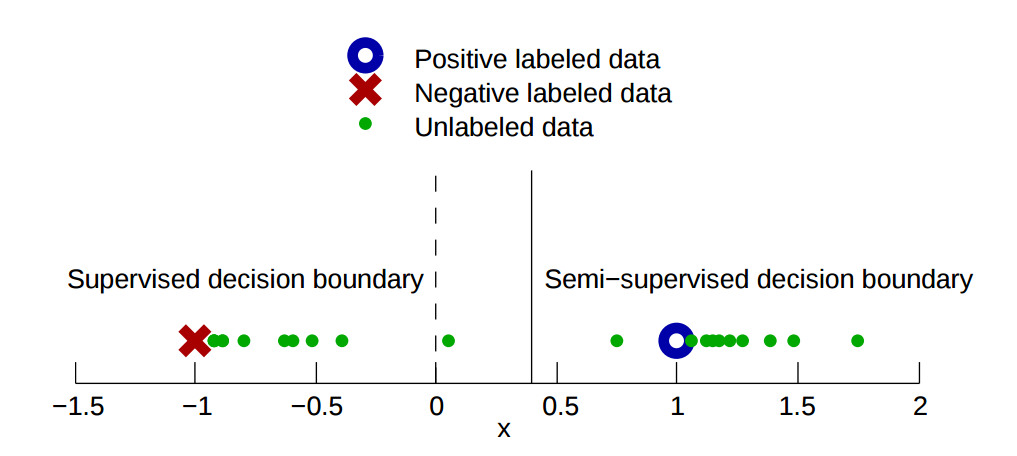
\includegraphics[width=10cm]{ssl.png}
\end{figure}

Co-training \cite{blum1998combining} is a semi-supervised learning technique that requires two
views of the data. It assumes that each example is described using two
different feature sets that provide different, complementary
information about the instance. Co-training first learns a separate
classifier for each view using any labeled examples. The most
confident predictions of each classifier on the unlabeled data are
then used to iteratively construct additional labeled training
data. The details of co-training algorithm is described in Algorithm~\ref{algo:co-training}.
\begin{algorithm}[h] \label{algo:co-training}
  \SetKwInOut{Input}{Input}
  \Input{labeled data $\left \{ (\mathbf{x}_i, y_i)
\right \}_{i=1}^{l}$, unlabeled data $\left \{ \mathbf{x}_j
\right \}_{j=l+1}^{l+u}$ \\
each instance has two views $\mathbf{x}_i=\left [ \mathbf{x}_i^{(1)},
  \mathbf{x}_i^{(2)} \right ]$ \\
and a learning speed $k$
}
Let $L_1 = L_2 = \left \{ (\mathbf{x}_1, y_1), \ldots, (\mathbf{x}_l, y_l)
\right \}.$ \\
\Repeat {unlabeled data is used up}{
  Train view-1 $f^{(1)}$ from $L_1$, view-2 $f^{(2)}$ from $L_2$ \\
  Classify unlabeled data with $f^{(1)}$ and $f^{(2)}$ separately. \\
  Add $f^{(1)}$'s top $k$ most-confident predictions $(\mathbf{x},
  f^{(1)}(\mathbf{x}))$ to $L_2$ \\
  Add $f^{(2)}$'s top $k$ most-confident predictions $(\mathbf{x},
  f^{(2)}(\mathbf{x}))$ to $L_1$ \\
  Remove these from the unlabeled data.
}

\caption{Co-training Algorithm for Semi-Supervised Learning}
\end{algorithm}

There are three important assumptions which guarantee the performance of
co-training algorithm: 1). feature split $x=[x^{(1)};x^{(2)}]$
exists; 2). $x^{(1)}$ or $x^{(2)}$ alone is sufficient to train a good
classifier; 3). $x^{(1)}$ and $x^{(2)}$ are conditionally independent
given the class.
\bibliographystyle{plain}
\bibliography{references}
\end{document}

%%% Local Variables:
%%% mode: latex
%%% TeX-master: t
%%% End:
